\documentclass[a4paper,11pt]{amsart} 
\usepackage[top = 2.5cm, bottom = 2.5cm, left = 2.5cm, right = 2.5cm]{geometry} 

\usepackage[T1]{fontenc}
\usepackage{hyperref}
\usepackage[utf8]{inputenc}
\usepackage{algorithm,algpseudocode}
\usepackage{float}
\usepackage{amsthm}
\usepackage{amsmath}
\usepackage{xcolor}
\usepackage{mathtools}
\usepackage{tikz}
\usepackage{pgfplots}
\usepackage{multirow} 
\usepackage{booktabs}
\usepackage{graphicx}

\usepackage{setspace}
\usepackage{float}
\usepackage{fancyhdr}
\usepackage{mathtools}

\pagestyle{fancy}
\fancyhf{}

\setlength{\parindent}{0in}

\title{The Contact Process}
\author{Michael Markl}
\date{December 8, 2020}

\newtheorem{proposition}{Proposition}
\newtheorem{theorem}{Theorem}
\bibliographystyle{plain}

\newcommand{\todo}[1]{\textcolor{red}{#1}}
\newcommand{\Cont}{C}
\newcommand{\diff}{\,\mathrm{d}}

\DeclareMathOperator{\LGen}{\mathcal{L}}

\DeclarePairedDelimiter\abs{\lvert}{\rvert}%
\DeclarePairedDelimiter\trin{\lvert\lvert\lvert}{\rvert\rvert\rvert}%
\DeclarePairedDelimiter\ceil{\lceil}{\rceil}
\DeclarePairedDelimiter\floor{\lfloor}{\rfloor}

\begin{document}

\thispagestyle{empty}
\maketitle

\section{Introduction and Preliminaries}

Contact processes are special spin-flip systems which can used to model, for example, the spread of an infection.
In the general case, we are given a countable, undirected graph $G=(S,E)$ of bounded degree $\deg_{\max}\coloneqq \sup_{x\in S} \deg(x) < \infty$.
The nodes of the graph are usually called \emph{sites} and during the contact process sites are either \emph{infected} or \emph{healthy}.
Hence, the state space of the process we are about to define is $\Omega\coloneqq \{0, 1\}^S$ where $0$ should be interpreted as healthy and $1$ as infected.

We denote sites by letters $x,y \in S$, configurations by $\eta, \zeta, \xi\in\Omega$.
The resulting configuration for flipping site $x$ in configuration is denoted as $\eta^x$ and two sites $x$ and $y$ are called \emph{neighboring} ($x \sim y$) if $\{x,y\}$ is an edge in $E$.

In a contact process, an infected site becomes healthy with after a unit exponential time.
On the contrary a healthy site becomes infected proportionally to the number of infected neighbors.
This proportionality coefficient $\lambda > 0$ is independent of the site itself.
Now we can define the flip rates of a site $x$ in a configuration $\eta$ by $$c(x,\eta) \coloneqq \begin{cases}
	1 & \text{if $\eta(x) = 1$,} \\
	\lambda \cdot \abs{ \{ y\sim x \mid \eta(y) = 1 \} } & \text{if $\eta(x) = 0$.}
\end{cases}$$

As any other spin system, these spin rates can be translated into a continuous time Markov chain with $Q$-Matrix of the form $q(\eta, \eta^x) \coloneqq c(x,\eta)$ and generator
$$
\LGen f(\eta) \coloneqq \sum_{x\in S} c(x,\eta) \left( f(\eta^x) - f(\eta) \right),
$$
if $M\coloneqq \sup_{x\in S} \sum_{u:x\neq u} \gamma(x,u) < \infty$ holds where $\gamma(x,u)\coloneqq \sup_{\eta\in\Omega} \abs{ c(x,\eta^u) - c(x,\eta) }$.
Here, this is indeed the case:
For $u\sim x$ we have $\gamma(x,u)=\lambda$, otherwise $\gamma(x,u)$ vanishes implying $M = \lambda \cdot \deg_{\max}$.
By looking at the $(M<\epsilon)$-Theorem with $\epsilon\coloneqq \inf_{x\in S, \eta\in \Omega} c(x,\eta)+ c(x,\eta^x) = 1$, we get the following result:
If  $\lambda <\deg_{\max}^{-1}$, then $\eta_t$ is \emph{ergodic}, i.e. there is a unique stationary distribution $\mu$ and for every $\eta\in\Omega$ and $f\in \Cont(\Omega)$ it fulfills $\lim_{t\to\infty} S_t f(\eta) = \int_\Omega f \diff \mu,$
where $S_t$ denotes the semigroup generated by $\LGen$.
As the pointmass $\delta_0$ on $0$ is always an invariant measure, we discuss in the next sections whether there are more invariant measures for $\lambda \geq \deg_{\max}^{-1}$.


Before that, we note, that any contact process is an \emph{attractive spin system}: If $\eta \leq \zeta$ holds component-wise, we have $c(x,\eta) = \lambda \cdot \abs{ \{ y\sim x\mid \eta(y) = 1 \}}\leq \lambda \cdot \abs{\{ y\sim x\mid \zeta(y) = 1 \}} = c(x,\zeta)$ for $\eta(x) = 1$ and $c(x, \eta) = 1 \leq 1 = c(x,\zeta)$ for $\zeta(x)=0$.
From the theory of attractive spin systems we know the existence of a lower invariant measure $\underline{\nu}\coloneqq \lim_{t\to\infty} \delta_0 S_t$
and an upper invariant measure $\overline{\nu} \coloneqq \lim_{t\to\infty} \delta_1 S_t$.
As $\delta_0$ is already invariant, $\underline{\nu} = \delta_0$ follows immediately.
The structure of $\overline{\nu}$ is less obvious for $\lambda \geq \deg_{\max}^{-1}$ as we will see in the next sections.


\section{The Graphical Representation}
\begin{figure}\label{fig:graphical-rep}
\caption{Graphical Representation of the contact process}
\vspace{1em}
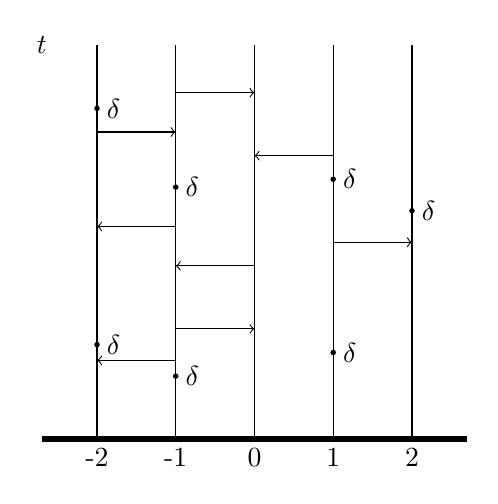
\begin{tikzpicture}
	\draw[line width=2pt] (-2.7,0) -- (2.7,0);
	
	\foreach \x in {-2, -1, ..., 2} {
		\node at (\x,0) [below] {\x};
		\draw (\x,0) -- (\x, 5);
	}
	
	\fill (-2,1.2) circle (1pt) node [right] {$\delta$};
	\fill (-2,4.2) circle (1pt) node [right] {$\delta$};
	
	\fill (-1,0.8) circle (1pt) node [right] {$\delta$};
	\fill (-1,3.2) circle (1pt) node [right] {$\delta$};
	
	\fill (1,1.1) circle (1pt) node [right] {$\delta$};
	\fill (1,3.3) circle (1pt) node [right] {$\delta$};
	
	\fill (2,2.9) circle (1pt) node [right] {$\delta$};
	
	\draw[->] (-2, 3.9) -> (-1,3.9);
	\draw[->] (-1, 2.7) -> (-2,2.7);
	\draw[->] (-1, 1.0) -> (-2,1.0);
	\draw[->] (-1, 4.4) -> (0,4.4);
	\draw[->] (-1, 1.4) -> (0,1.4);
	\draw[->] (0, 2.2) -> (-1,2.2);
	\draw[->] (1, 3.6) -> (0,3.6);
	\draw[->] (1, 2.5) -> (2,2.5);
	
	\node at (-2.7, 5) {$t$};
\end{tikzpicture}
\end{figure}

\section{Critical Values for Survival}



\section{The Contact Process on Homogeneous Trees}


\section{More Results}


\end{document}